%% 
%% Template chap2.tex
%% 

\chapter{Methodology}
\label{cha:methodology}

\section{Lower Linear Envelope MRFs}
\label{sec:inference}

We begin with extending standard Markov Random Fields (see
equation~\eqref{eq:energyfunction_UPH}) to include the lower
linear envelope potential. We then show how to perform exact
inference in models with these potentials. In \ref{sec:learning}
we will discuss learning the parameters of the models. Major
work in this section is done by \citename{gouldlearning}.

% \subsection{Lower Linear Envelope Potentials}
% \label{sec:llep}
% From section~\ref{sec:MRF} we have already introduced that an
% \emph{energy function} may contain \emph{unary}, \emph{pairwise}
% and \emph{higher-order} potentials (see
% equation~\eqref{eq:energyfunction_UPH}). In this section we
% mainly focus on one class of higher-order potentials $\phi^H$
% defined as a concave piecewise linear function which is known as
% \emph{lower linear envelope potentials}. This has been studied
% extensively in Markov Random Fields area for encouraging
% consistency over large
% cliques~\cite{Kohli:CVPR07,Nowozin:2011,Gould:ICML2011}.

% Let $\C$ denotes the set of all maximal cliques in an image and
% $\by_c=\{y_i |\text{\,for\,} i \in c\}$ denotes set of random
% variables in the clique $c$, a weighted lower linear envelope
% potential~\cite{gouldlearning} over $\by_c$ is defined as the
% minimum over a set of $K$ linear functions as:
% %
% \begin{align}
%   \psi^H_c\!(\by_c) \, &= \min_{k=1, \ldots, K} \left\{ a_k W_{\!c}(\by_c) + b_k \right\}.
%   \label{eqn:potential2}
% \end{align}
% %
% where $W_{\!c}(\by_c) = \sum_{i \in c} w_i y_i$ with $w^c_i \geq
% 0$ and $\sum_{i \in c} w^c_i = 1$ which are weights for each
% clique. $(a_k, b_k) \in \reals^2$ are the linear function
% parameters. We illustrate an example~\cite{gouldlearning} with
% three linear functions in \figref{fig:nonredundant}.
% %
% \begin{figure}[ht]
%   \centering
%   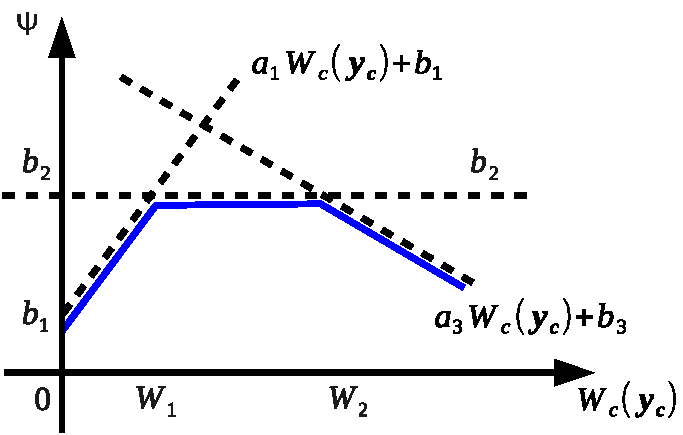
\includegraphics[width=0.6\columnwidth]{Methodology/figures/not_redundant}
%   \caption{\label{fig:nonredundant} Example lower linear envelope
%     $\psi^H_c\!(\by_c)$ (shown solid) with three terms (dashed).
%     When $W_{\!c}(\by_c) \leq W_1$ the first linear function is
%     active, when $W_1 < W_{\!c}(\by_c) \leq W_2$ the second
%     linear function is active, otherwise the third linear
%     function is active.}
% \end{figure}

% Inference on energy function contains lower linear potentials is
% the same as the standard equation~\eqref{eq:energyfunction_UPH}
% and is given by:
% \begin{align}
%   \label{eq:min_energy}
%   \by^* = \argmin\energy{\by}
% \end{align}

% \begin{figure}[ht]
%   \centering
%   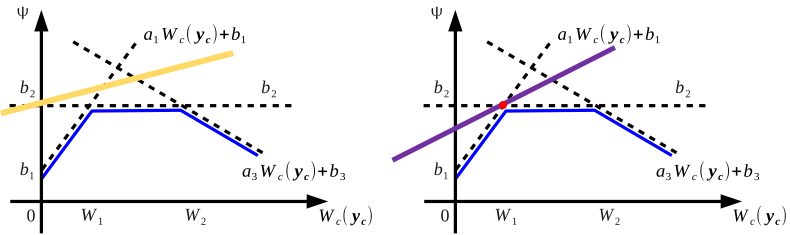
\includegraphics[width=1\columnwidth]{Methodology/figures/redundant}
%   \caption{\label{fig:redundant} Example lower linear envelope
%     with redundant linear functions. On the left figure, the
%     solid yellow line is always inactive. On the right figure,
%     the solid purple line intersects $line \; 1$ and $line \; 2$
%     at the red point. It's only active when $line \; 1$ and $line
%     \; 2$ are both active. Both solid lines are redundant linear
%     functions hence can be removed without changing their energy
%     function.}
% \end{figure}
% %
% Suppose that parameters $\{(a_k, b_k)\}_{k=1}^K$ are sorted in
% decreasing order of $a_k$. From \emph{Definition 3.1}
% \cite{gouldlearning} we know that the $k$-th linear function is
% said to be \emph{active} if there exists $x \in (0, 1)$ such that
% the following two inequalities hold
% \begin{align}
%   a_{k-1} x + b_{k-1} &> a_k x + b_k \nonumber \\
%   a_{k+1} x + b_{k+1} &> a_k x + b_k
%   \label{eqn:nonred_in_ab}
% \end{align}
% %
% The $k$-th linear function is said to be \emph{redundant}
% (\emph{Definition 3.2}~\cite{gouldlearning}) if it is not active
% for any assignment to $\by_c$ in any clique $c \in \C$ or is only
% active whenever another linear function is also active.
% Figure \ref{fig:redundant} depicts such conditions. As a
% result, removing redundant functions from the potential does not
% chang the energy function.

% To ensure potentials do not contain redundant linear functions,
% \citename{gouldlearning} rearranged conditions
% \ref{eqn:nonred_in_ab} in terms of $x$ and proposed a condition on
% parameters of the envelope. The $k$-th linear function is
% not redundant if the following condition is satisfied:
% %
% \begin{align}
%     0
%     <
%     \frac{b_k - b_{k-1}}{a_{k-1} - a_k}
%     <
%     \frac{b_{k+1} - b_k}{a_k - a_{k+1}}
%     <
%     1.
%   \label{eq:nonredundant}
% \end{align}
% %
% Another important property of equation~\eqref{eq:min_energy} is
% shift invariant~\cite{gouldlearning} (vertically). We write
% $\widetilde{\psi}^{H}_c\!(\by_c)$ by shift equation~\eqref{eqn:potential2} vertically
% with an abitrary amount $b^{const}\in R$
% $$\widetilde{\psi}^{H}_c\!(\by_c) = \min_{k=1, \ldots, K}
% \left\{a_k W_{\!c}(\by_c) + b_k + b^\textrm{const} \right\}$$
% %
% Then we have
% \begin{align}
%   \argmin_{\by_c} \psi^H_c\!(\by_c)
%   = \argmin_{\by_c} \widetilde{\psi}^{H}_c\!(\by_c).
%   \label{eq:shift_invariant}
% \end{align}
% %
% Therefore, in the following discussion without loss of generality
% we assume $b_1 = 0$ thus $b_k\geq0 \text{\; for \;} k=1,\dots,n$.
% %
\subsection{Exact Inference}
\label{sec:exact_inference}

Exact inference on MRFs has been extensively studied in past
years. Researchers found that, energy functions which can be
transformed into quadratic pseudo-Boolean
functions~\cite{Ishikawa:PAMI03,Ishikawa:CVPR09,Rother:CVPR09}
are able to be minimized exactly using \emph{graph-cuts} like
algorithms~\cite{Freedman:CVPR05,Hammer:1965} when they satisfy
submodularity condition~\cite{Boros:MATH02}.
\citename{Kohli:TR08} and \citename{Gould:ICML2011} adapted those
results to perform exact inference on lower linear envelope
potentials. In this section we mainly focus on describing the
\emph{st min cut} graph constructed by
Gould~\cite{Gould:ICML2011,gouldlearning} for exact
inference~\eqref{eq:min_energy} of energy function containing
lower linear envelope potentials.

Following the approach of \citename{Kohli:CVPR10},
\citename{Gould:ICML2011,gouldlearning} transformed the weighted
lower linear envelope potential~\eqref{eqn:potential2} into a
quadratic pseudo-Boolean function by introducing $K-1$ auxiliary
variables $\bz = \left(z_1, \ldots, z_{K-1}\right)$ with $z_k\in
\{0,1\}$:

\begin{align}
  E^c(\by_c, \bz) = a_1 W_{\!c}(\by_c) + b_1
  {}+ \sum_{k = 1}^{K-1} z_k \left( \left(a_{k+1} - a_k\right) W_{\!c}(\by_c) + b_{k+1} - b_k \right)
  \label{eqn:binary_concave_z}
\end{align}

\noindent for a single clique $c \in \C$. Under this formulation,
\citename{Gould:ICML2011,gouldlearning} showed that minimizing
the pseudo-Boolean function over $\bz$ is equivalent to selecting
(one of) the active functions(s) from
equation~\eqref{eqn:potential2}. Another important property of
optimized $\bz$ under this formulation is that it
automatically satisfies the constraint~\cite{gouldlearning}: 

\begin{figure}[t]
  \centering
  \setlength{\tabcolsep}{2pt}
  \begin{tabular}{cc}
    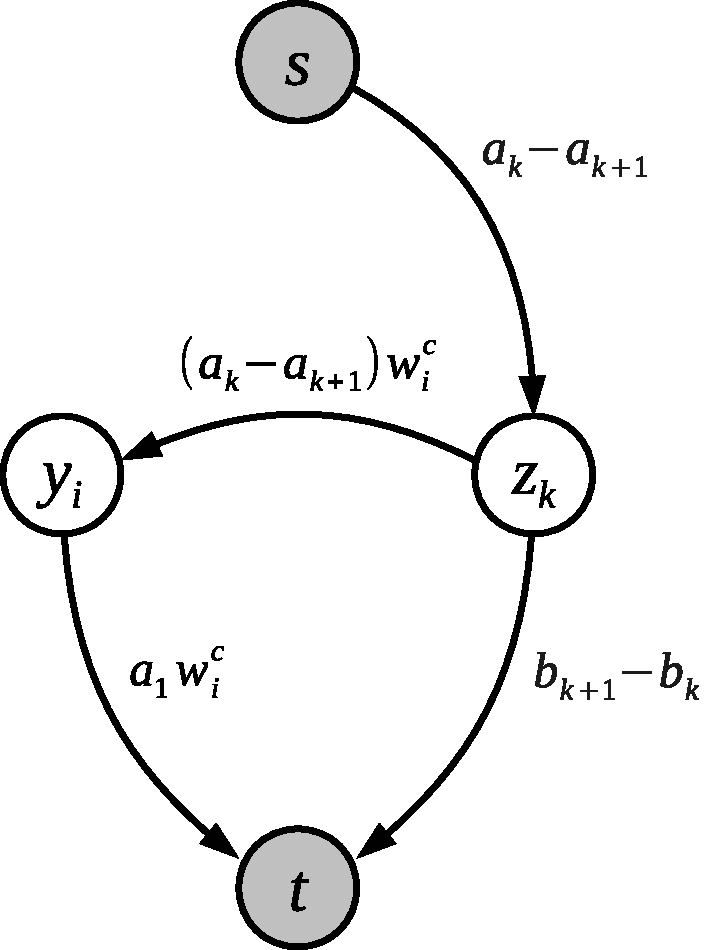
\includegraphics[width=0.45\columnwidth]{Methodology/figures/stmincut}&
                                                                         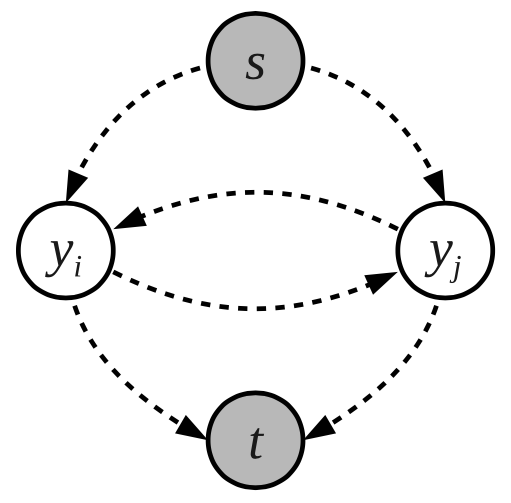
\includegraphics[width=0.5\columnwidth]{Methodology/figures/unary_pairwise.png}\\
                                                                         {\small (a)} & {\small (b)} 
  \end{tabular}
  \caption{\label{fig:stmincut} $st$-graph
    construction~\cite{gouldlearning} for
    equation~\eqref{eqn:posiform}, unary and pairwise terms.
    Every cut corresponds to an assignment to the random
    variables, where variables associated with nodes in the
    ${\cal S}$ set take the value one, and those associated with
    nodes in the $\T$ set take the value zero. With slight abuse
    of notation, we use the variables to denote nodes in our
    graph.}
\end{figure}

\begin{align}
  \label{eq:z_consecutive_constraint}
  z_{k+1} \leq z_k
\end{align}

\noindent this property give rise to further development of
parameter vector~\eqref{eq:llsvm_param} and feature
vector~\eqref{eq:llsvm_feature} which are used in latent
structural SVM.

In order to construct the \emph{st-min-cut} graph,
\citename{gouldlearning} rewrote
equation~\eqref{eqn:binary_concave_z} into
\emph{posiform}~\cite{Boros:MATH02}:

\begin{align}
  \label{eqn:posiform}  
  E^c(\by_c, \bz)
  &= b_1 - (a_1 - a_K) + \sum_{i \in c} a_1 w^c_i y_i
  {}+ \sum_{k = 1}^{K - 1} \left( b_{k+1} - b_k \right) z_k\\
  &+ \sum_{k = 1}^{K - 1} \left( a_k - a_{k+1} \right) \bar{z}_k
  {}+ \sum_{k = 1}^{K - 1} \sum_{i \in c} \left( a_k - a_{k+1}
    \right) w^c_i \bar{y}_i z_k \nonumber
\end{align}

\noindent where $\bar{z}_k = 1 - z_k$ and $\bar{y}_i = 1 - y_i$.
$a_1$ is assumed to be greater than $0$ so that all coefficients
are positive (recall we assume $b_1=0$ in section~\ref{sec:llep}
and we have $a_k > a_{k+1}$ and $b_k < b_{k+1}$). After proving
\emph{submodularity} of the energy function~\eqref{eqn:posiform},
\citename{gouldlearning} constructed the \emph{st-min-cut} graph
based on equation~\eqref{eqn:posiform}.

The construction is explained in \figref{fig:stmincut}. Figure
(a) denotes construction for equation~\eqref{eqn:posiform}. For
each lower linear envelope potential edges are added as follows:
for each $i \in c$, add an edge from $y_i$ to $t$ with weight
$a_1 w^c_i$; for each $i \in c$ and $k = 1, \ldots, K-1$, add an
edge from $z_k$ to $y_i$ with weight $(a_{k} - a_{k+1}) w^c_i$;
and for $k = 1, \ldots, K-1$, add an edge from $s$ to $z_k$ with
weight $a_k - a_{k+1}$ and edge from $z_k$ to $t$ with weight
$b_{k+1} - b_k$. Figure (b) denotes construction for unary and
pairwise terms (see \cite{Kolmogorov:PAMI04}). For unary edges (4
edges on both sides), weights on each edge are corresponding to
values in input unary terms accordingly. For pairwise edges (2
edges in the middle), both edges share the same weight which
equals to the input pairwise term.

\section{Learning the Lower Linear Envelope with Latent Information}
\label{sec:learning}

With the inference algorithm in hand, we now can develop the
learning algorithm for weighted lower linear envelope potentials
using the latent structural SVM framework. We begin by
transforming the equation~\eqref{eqn:binary_concave_z} into a
linear combination of parameter vector and feature vector. Then a
two-step algorithm was developed to solve the latent structural
SVM.


% \subsection{Transforming Between Representations}
% \label{sec:latent_linEnv_represent}

% The latent structural SVM formulation (see
% equation~\eqref{eq:latent_ssvm_linearcomb}) requires that the
% energy function be expressed as a linear combination of features
% and weights while our higher-order potential is represented as
% the minimum over a set of linear functions. However,
% in~\ref{sec:exact_inference} we reformulated the piesewise linear
% functions into a quadratic pseudo-Boolean
% function~\eqref{eqn:binary_concave_z} by introducing auxiliary
% variables. Now we show function~\eqref{eqn:binary_concave_z}
% itself is an inner product of parameter vector and feature vector
% with latent information. We first noticed that the function can
% be expanded as a summation of $2K-1$ terms:

% \begin{align}
%   \label{eq:originalenergy}
%   E^c(y_c,z)&=a_1W_c(y_c)+b_1+\sum_{k=1}^{K-1}z_k((a_{k+1}-a_k)W_c(y_c)+b_{k+1}-b_k)\nonumber\\ 
%             &=a_1W_c(y_c)+\sum_{k=1}^{K-1}(a_{k+1}-a_k)z_kW_c(y_c)+\sum_{k=1}^{K-1}(b_{k+1}-b_k)z_k
% \end{align}

% Here we use the fact of equation~\eqref{eq:shift_invariant} and
% let $b_1=0$. Now we can reparameterize the energy function
% as
% \begin{align}
%   \label{eq:llsvm_innerprod_energy}
%   E^c(\by_c,\bz; \btheta) = \btheta^T \! \phi(\by_c,\bz)
% \end{align}

% \noindent where:

% \begin{equation}
% \label{eq:llsvm_param}
%   \theta_k = \left\{
%     \begin{aligned}
%       & a_1	& \text{for} \ k=1\\
%       & a_k-a_{k-1} & \text{for}\ 1< k \leq K\\
%       & b_{k+1-K}-b_{k-K} & \text{for} \ K<k\le2K-1\\
%     \end{aligned}
%   \right.
% \end{equation}

% \begin{equation}
% \label{eq:llsvm_feature}
%   \phi_k = \left\{
% 		\begin{aligned}
%       & W_c(\by_c) 	& \text{for} \ k=1\\
%       & W_c(\by_c)\bz_k & \text{for}\ 1<k\le K\\
%       & \bz_k & \text{for} \ K<k\le2K-1\\
% 		\end{aligned}
%   \right.
% \end{equation}

% Under this formulation, inference
% problems~\eqref{eq:latentssvm_full_inf}
% and~\eqref{eq:latentssvm_latent_inf} introduced in
% section~\ref{sec:latent-struct-svms} can be written as:

% \begin{align}
%   \label{eq:linenv_full_inf}
%   (\mathbf{\hat{y}}_k(\btheta),\mathbf{\hat{z}}_k(\theta))=\argmin_{(\mathbf{y}
%   \times \mathbf{z}) \in \mathcal{Y} \times \mathcal{Z}}
%   \btheta^T\cdot\phi(\mathbf{y}_k,\mathbf{z}_k)
% \end{align}
% and
% \begin{align}
%   \label{eq:linenv_latent_inf}
%   \mathbf{z}^*_k(\btheta) = \argmin_{\mathbf{z} \in \mathcal{Z}}
%   \btheta^T \cdot \phi(\mathbf{y}_k,\mathbf{z}_k)
% \end{align}

% There are 2 facts worth to mention. The first fact is
% that in our previous construction of minimum-$st$-cut graph the
% latent variable $\bz$ is already included. Therefore, we can
% apply our inference algorithm directly on our 2 new formulations.

% However, for equation~\eqref{eq:linenv_latent_inf} there exists
% more efficient algorithm. At training stage the ground-truth
% labels $y_i$ is a function input thus completely observed.
% Therefore, the term $((a_{k+1}-a_k)W_c(\by_c)+b_{k+1}-b_k)$ in
% equation~\ref{eq:originalenergy} becomes constant. So we can
% infer latent variable $\bz$ explicitly by:
% \begin{align}
%   \label{eq:linenv_effi_infer_latent}
%   z_k^c &=
%           \begin{cases}
%             0 & \text{if $((a_{k+1}-a_k)W_c(y_c)+b_{k+1}-b_k)\geq0$} \\
%             1 & \text{otherwise}.
%           \end{cases}
% \end{align}

% \begin{figure}[t]
%   \centering
%   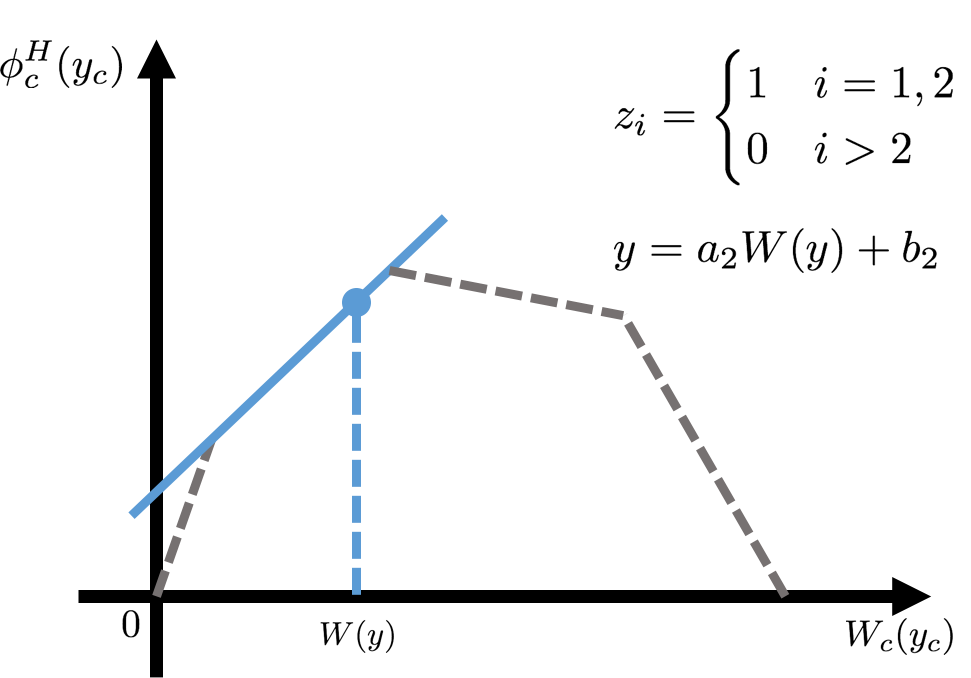
\includegraphics[width=0.8\columnwidth]{Methodology/figures/linEnvLatentFig.png}
%   \caption{\label{fig:concave} Example piecewise-linear concave
%     function of $W_{\!c}(\by_c) = \sum_{i \in c} w^c_i y_i$.
%     Assume the second linear function is active namely
%     $\bz^c=(1,1,0,0)$. The result of linear combination of
%     parameter vector and feature vector is same as quadratic
%     psuedo-Boolean function.}
% \end{figure}

% To show the equivalence between
% equation~\eqref{eqn:binary_concave_z} and
% equation~\eqref{eq:llsvm_innerprod_energy} we consider the
% example illustrated in figure~\ref{fig:concave}. Assume the
% inferred latent vector $\bz^c=(1,1,0,0)$. Plug it into
% equation~\eqref{eq:llsvm_feature} the energy function can be
% written as:
% \begin{align*}
%   E^c(\by_c,\bz; \btheta) &=
%   \begin{bmatrix}
%     a_1\\
%     a_2-a_1\\
%     a_3-a_2\\
%     a_4-a_3\\
%     b_2\\
%     b_3-b_2\\
%     b_4-b_3
%   \end{bmatrix}^T
%   \begin{bmatrix}
%     W_c(\by_c) \\
%     W_c(\by_c) \\
%     0\\
%     0\\
%     1\\
%     0\\
%     0
%   \end{bmatrix}\\
%   &=a_1W_c(\by_c)+(a_2-a_1)W_c(\by_c)+b_2\\
%   &=a_2W_c(\by_c)+b_2
% \end{align*}

% Therefore, assignments inferred by graph-cut algorithm can be
% directly encoded into a linear combination by using our latent
% structural SVM formulation for learning purpose. The remaining
% task is to ensure the concavity of $\btheta$. We do this by
% adding the following constraint:

% \begin{align}
%   A\btheta\geq0 \text{,\;~~~} A=
%                   \begin{bmatrix}
%                     1 & \mathbf{0} & \mathbf{0}\\
%                     \mathbf{0} & -\mathbf{1} & \mathbf{0}\\
%                     \mathbf{0} & \mathbf{0} & \mathbf{P}
%                   \end{bmatrix}\in \mathbb{R}^{(2K-1)\times(2K-1)}
% \end{align}

% \noindent where $-\mathbf{1}$ is a matrix of size $(K-1)\times(K-1)$ and
% $\mathbf{P}$ is an identity matrix of size $(K-1)\times(K-1)$.

% One subtle problem we found during experiments is that the
% algorithm can be stuck small numerical value. To avoid this we
% add small slack variables $\epsilon$ on those constraints:

% \begin{align}
%   \label{eq:concave_constraint}
%   A\btheta\geq\epsilon \text{,\;~~~} A=
%                   \begin{bmatrix}
%                     1 & \mathbf{0} & \mathbf{0}\\
%                     \mathbf{0} & -\mathbf{1} & \mathbf{0}\\
%                     \mathbf{0} & \mathbf{0} & \mathbf{P}
%                   \end{bmatrix}\in \mathbb{R}^{(2K-1)\times(2K-1)}
% \end{align}

% \noindent where $\epsilon$ usually equal to $\mathbf{1}^{-15}$ in our
% experiments.

% % \subsection{Latent Structural SVM Learning}
% % \label{sec:mrflssvm_learning_algo}

% % With the inner product formulation
% % (equation~\eqref{eq:llsvm_innerprod_energy}) of higher order
% % energy function in hand, we now able to develop our latent
% % structural SVM learning algorithm. The energy function (higher
% % order function together with unary and pairwise functions) can be
% % written as:
% % \begin{equation}
% %   E_{all}(y,z) = \begin{bmatrix}
% %     \btheta^H\\
% %     \theta^{unary}\\
% %     \theta^{pairwise}
% %   \end{bmatrix}^T 
% %   \cdot \begin{bmatrix}
% %     \phi^H\\
% %     \phi^{unary}\\
% %     \phi^{pairwise}
% %   \end{bmatrix}=\theta_{all}^T\cdot\phi_{all}
% % \end{equation}
% % where $\btheta^H\in \real$ is the parameter vector in higher
% % order equation~\eqref{eq:llsvm_innerprod_energy} of size $2K-1$.
% % $\theta^{unary}$ and $\theta^{pairwise}$ are both scalars.
% % $\phi^\textrm{unary} = \sum_i \psi^U_i\!(y_i)$ and
% % $\phi^\textrm{pairwise} = \sum_{ij} \psi^P_{ij}(y_i, y_j)$.
% % Therefore, the size of $\theta_{all}$ is $2K+1$.

% % Plug equation~\eqref{eq:linenv_full_inf} and
% % equation~\eqref{eq:linenv_latent_inf} into object
% % function~\eqref{eq:latent_ssvm_object}, the latent structural SVM
% % object function for our problem can be derived as a difference of
% % two convex functions:

% % \begin{align}
% % \label{eq:lssvm_object}
% %   \min_\theta\bigg(\frac{1}{2}\|\theta\|^2+
% %   C\sum_{i=1}^{n}\big(\max_{(\mathbf{\hat{y}} \times
% %   \mathbf{\hat{z}}) \in \mathcal{Y} \times \mathcal{Z}}
% %   [\theta\cdot\phi(\mathbf{\hat{y}},\mathbf{\hat{z}}) +
% %   \Delta(\mathbf{y}_i,\mathbf{\hat{y}},\mathbf{\hat{z}})]\big)\bigg)\\
% %   -C\sum_{i=1}^{n}\big(\max_{\mathbf{z} \in \mathcal{Z}} \theta \cdot
% %   \phi(\mathbf{y}_i,\mathbf{z})\big)\nonumber
% % \end{align}

% % As mentioned by \citename{yu2009learning} the Concave-Convex
% % Procedure (CCCP)~\cite{yuille2002concave} can be used to solve the
% % optimization problem. Our algorithm contains two stages. We first
% % imputes the latent variables $\bz$ explicitly by
% % equation~\eqref{eq:linenv_latent_inf}. Namely solving the
% % ``latent variable completion'' problem~\cite{yu2009learning}:

% % \begin{align}
% %   \bz_i^*=\argmax_{\mathbf{z} \in \mathcal{Z}} \theta \cdot
% %   \phi(\mathbf{y}_i,\mathbf{z})
% % \end{align}

% % The inference result $z_i^*$ for $i=1,\dots,n$ is used as
% % completely observed for later stage. With the latent variable
% % $z_i^*$ which best explains the ground-truth data $y_i$ in hand,
% % updating the parameter vector $\btheta$ is similar to solve the
% % standard max-margin optimization problem described
% % in~\cite{gouldlearning}:

% % \begin{align}
% % \label{eq:mrflssvm_object}
% %   \min_\theta\bigg(\frac{1}{2}\|\theta\|^2+
% %   C\sum_{i=1}^{n}\big(\max_{(\mathbf{\hat{y}} \times
% %   \mathbf{\hat{z}}) \in \mathcal{Y} \times \mathcal{Z}}
% %   [\theta\cdot\phi(\mathbf{\hat{y}},\mathbf{\hat{z}}) +
% %   \Delta(\mathbf{y}_i,\mathbf{\hat{y}},\mathbf{\hat{z}})]\big)\bigg)\\
% %   -C\sum_{i=1}^{n}\big(\theta \cdot
% %   \phi(\mathbf{y}_i,\mathbf{z}_i^*)\big) \nonumber
% % \end{align}

% % The last problem remaining is the initialization method. Because
% % our objective function~\eqref{eq:mrflssvm_object} is not convex
% % and the CCCP algorithm is only guaranteed to converge to a local
% % minimum or saddle point\cite{yuille2002concave}, initialization
% % of $\btheta$ might affect the performance of our algorithm. Since
% % there are no theoretical solution for this problem, we only
% % propose an empirical \algref{alg:init_theta}:

% % \begin{algorithm}[ht]
% %   \begin{algorithmic}[1]
% %     \STATE{$gap=\frac{1}{K}$, $a_1=\U(0,1e6)$, $b_1=0$,
% %       $sp_1=(0,0)$, $w_0=0$, $counter=2$} \FOR{each
% %       clique $c\in \C$} \STATE{Compute weighted clique value
% %       $w_c=W_c(y_C)$} \IF{$w_c-w_{c-1}>gap$}
% %     \STATE{$upbound = a_{counter}w_c+b_{counter}$\\
% %       $sp_{counter}=(w_c,\U(upbound-0.5,upbound))$\\
% %       Calculate $a_{counter}$ and $b_{counter}$ using
% %       $sp_{counter-1}$ and $sp_{counter}$\\
% %       $counter=counter+1$}
% %     \ENDIF
% %     \ENDFOR
% %     \STATE{If $counter<K$, remaining $a$s and $b$s are all set to
% %       be $a_{counter}$ and $b_{counter}$} \STATE{Calculate
% %       $\btheta$ using $\{a_k,b_k\}_{k=1}^K$}
% %   \end{algorithmic}
% %   \caption{\label{alg:init_theta} Empirical initialization
% %     algorithm for $\btheta$}
% % \end{algorithm}

% % We assume that the more evenly distributed of $W_c(Y_c)$ where
% % $c\in\C$ on $x$ axis, the more rich representation (number of
% % linear functions) the energy function should have. In order to
% % initialize $\btheta$, we first determine the x-coordinate of
% % sampled points $sp$. Then we sample its y-coordinate from a
% % uniform distribution $\U(upbound,upbound-0.5)$ to add some
% % randomness in our initialization as well as maintain concavity.
% % Linear parameters $a_k$ and $b_k$ are later calculated using
% % those sampled points $sp_k$ and $sp_{k-1}$. At last we encode
% % $\{a_k,b_k\}_{k=1}^K$ into $\btheta$ using
% % equation~\eqref{eq:llsvm_param}.

% % Our optimization algorithm is summarized in
% % \algref{alg:learning}.

% % \begin{algorithm}[hb]
% %   \begin{algorithmic}[1]
% %     \STATE{Set $MaxIter = 100$}
% %     \STATE{ {\bf input} training set $\{\by_i\}_{i=1}^{n}$, regularization constant $C > 0$,
% %       and tolerance $\epsilon \geq 0$}
% %     \STATE{Initialize $\btheta$ using \algref{alg:init_theta}}
% %     \REPEAT
% %     \STATE{Set $iter = 0$}
% %     \FOR{each training example, $i = 1, \ldots, n$}
% %     \STATE{compute $ \bz_i^*=\argmax_{\mathbf{z} \in \mathcal{Z}}
% %       \theta \cdot \phi(\mathbf{y}_i,\mathbf{z}) $}
% %     \ENDFOR

% %     \STATE{ {\bf initialize} active constraints set $\C_i = \{ \}$ for all $i$}
% %     \REPEAT

% %     \STATE{solve the quadratic programming problem in
% %       equation~\ref{eq:mrflssvm_object} with respect to active
% %       constraints set $\C_i$ for all $i$ and concavity constraints
% %       $A\btheta\geq \epsilon$ to get
% %       $\hat{\btheta}$ and $\hat{\bxi}$}

% %     \FOR{each training example, $i = 1, \ldots, n$}
% %     \STATE{compute $\hat{\by_i},\hat{\bz_i} = \argmin_{\by}
% %       E(\by,\bz; \hat{\btheta}) - \Delta(\by, \bz, \by_i)$}
% %     \IF{$\hat{\xi}_i + \epsilon \!<\! \Delta(\hat{\by_i},
% %       \hat{\bz_i}, \by_i) -
% %       E(\hat{\by_i},\hat{\bz_i}; \hat{\btheta}) + E(\by_i, \bz_i^*; \hat{\btheta})$}
% %     \STATE{$\C_i \leftarrow \C_i \cup \{\by_i^\star\}$}
% %     \ENDIF
% %     \ENDFOR
% %     \UNTIL{no more violated constraints}
% %     \STATE{ {\bf return} parameters $\hat{\btheta}$}
% %     \STATE{Set $iter = iter+1$}

% %     \UNTIL{$iter\geq MaxIter$}
% %     \STATE{ {\bf return} parameters $\hat{\btheta}$}
% %   \end{algorithmic}
% %   \caption{\label{alg:learning} Learning lower linear envelope
% %     MRFs with latent variables.}
% % \end{algorithm}



% % \clearpage
% % \cleardoublepage


% % %%% Local Variables:
% % %%% mode: latex
% % %%% TeX-master: "../thesis"
% % %%% End:
